\documentclass[12pt]{article}
\usepackage{graphicx}
\graphicspath{{img/}}
\usepackage[left=0.8in,top=0.8in,right=0.8in,bottom=0.8in]{geometry}
\setlength\parindent{24pt}
\usepackage{titling}
\usepackage{gensymb}
\usepackage{enumitem}
\usepackage{sectsty}
\usepackage{float}
\sectionfont{\fontsize{12}{16}\selectfont}

\newlist{mylist}{enumerate}{1}%
\setlist[mylist]{label={[\arabic*]}}%

\title{\vspace{-3em} \textbf{Homework \#1}}

\author{Justin Kang \\ AST 381: Planetary Astrophysics}
\date{September 18, 2017}

\begin{document}
\maketitle


\section*{Introduction}
All code is found in \texttt{src/}, and will be referred to directly. The coding for this assignment was all done in Python (3.6.2). The \texttt{math}, \texttt{numpy}, \texttt{astropy}, and \texttt{matplotlib} libraries were all used for convenience in terms of constants, functions, time, and graphing. \texttt{main.py} is used as a script that sets all of the specific values for this project (such as using the HD 80606 system), for running the relevant scripts for each part, then generating output as necessary. For inputs of bodies in functions, the order is always first the affected body, then affecting/reference body. Whenever referring equations from the textbook (Sara Seager's \textit{Exoplanets}) in this report, the format will be ("Section numeral"."Chapter number"."Equation number"), and whenever referring to external links, [ ] will be used.


\section{Orbit Predictions}
For this portion of the project, the files of interest are \texttt{celestialbody.py}, \texttt{radialvelocity.py}, and \texttt{position.py}. First, \texttt{celestialbody.py} describes the class \texttt{CelestialBody} designed to make working with celestial bodies easier. It stores the mass and orbital elements of the body, as well as the radius (used in Section 3). The object-oriented design of this class allows for users to conveniently input their own values for testing code (prompting through IO) during construction, or for these bodies to be constructed directly with predetermined values. It also does input validation on IO, and stores internally all of the values in SI units. In \texttt{main.py} this is used to represent HD 80606 and its planetary companion and apply functions based on them and their properties. Here we see that the two bodies share almost all of their orbital elements, except they have a 180{\degree} offset in the argument of periapse (to conserve momentum).\\
\indent \texttt{radialvelocity.py} makes up the bulk of this section. The only public function is \\\texttt{radial\_velocity()}, which given two bodies and an initial and final time, returns a RV curve for the given time range. This is done by first calculating the orbital period using Kepler's third law (I.2.23). After doing so, a preset number of intervals are created within that time range, and the mean anomaly is calculated using these intervals (I.2.40). The Newton-Raphson method is employed to then calculate the eccentric anomaly (I.2.43). Afterwards, the true anomaly is calculated [1], then finally the radial velocity is calculated (II.1.11). Thus \texttt{radial\_velocity()} effectively changes radial velocity from function of true anomaly to a function of time. In the end, the function returns a tuple of the specific time intervals chosen (note: all functions described in this section and Section 3 will return a tuple of time intervals in JD and the desired value), and the radial velocities for those times (m/s). The choice of which RV curve is returned can be changed by just changing the order the bodies are inputted into the function.\\\\
\indent In \texttt{position.py}, the projected separation and position angles are calculated, for A with respect to B, and with respect to the center of mass. To calculate the projected separation of the planet with respect to the star, \texttt{projected\_separation()} is called. First the radius of the planet's orbit is calculated as a function of true anomaly (I.2.20), which is calculated as a function of time by borrowing a private function from \texttt{radialvelocity.py}. This is then used to calculate the projected coordinates (I.2.53-54). The projected coordinates are based using the star as the origin, thus the Pythagorean theorem is used to return the projected separation between the two bodies (AU). To get the projected separation of the planet and star with respect to the center of mass, \texttt{projected\_separation\_com()} is called. Here the position of the center of mass is calculated using the center of mass equation. Then the projected separation of the star is just that distance, and the projected separation of the planet is the original projected separation less that distance. To calculate the position angle of the planet with respect to the star, \texttt{position\_angle()} is used. This follows the same path as \texttt{projected\_separation()} up to calculating the coordinates. It then gets the position angle (degrees) by calculating the inverse tangent of Y over X. As X points directly north and Y directly east this is correct, and \texttt{arctan2()} is used to get the specific quadrant. Calculation of the position angles of both bodies with respect to the center of mass is quite simple, as seen in \texttt{position\_angle\_com()} - the position angle of the planet remains the same, and the star has a 180{\degree} offset (again, to conserve momentum).


\section{Extreme Planetary Orbits}
The parameters necessary to construct the \texttt{CelestialBody} objects for HD 80606 and its planet were obtained from the NASA Exoplanet Archive [2]. After constructing the two bodies, \\\texttt{radial\_velocity()} is called to obtain the RV curve of the star and the times of the maximum and minimum RV are printed. From this, the times of the RV maximum for this semester are JD 2457987.042 and 2458098.405, while the those for the RV minimum are 2457988.749 and 2458100.113. Converting these to local time for McDonald Observatory (CDT/CST), these are then August 21 8:00:28.8, August 23 0:58:33.6, December 10 15:43:12.0, and December 12 8:42:43.2. In order to measure the minimum, August 23 would have been the best date. Unfortunately for the max both times occur when the Sun is up, but August 21 would have resulted in much better data as the maximum doesn't occur in the middle of the day. Thus in order to (almost) measure the extreme maximum and minimum, one would want the nights of August 20 and 22. 

\begin{figure}[H]
\centering
\vspace{1em}
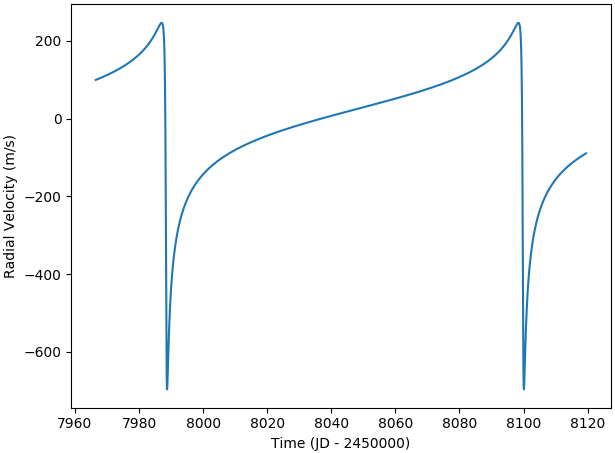
\includegraphics[width=0.8\textwidth]{rv.png}
\vspace{-1em}
\caption{The RV curve for HD 80606 during August-December 2017.}
\end{figure}


\section{Extreme Transits}
The code for this section can be found in \texttt{transit.py}. \texttt{transit()} calculates when the HD 80606 b transits its parent, if it at all. It does this by simply calling \texttt{projected\_separation()} - if the projected separation is smaller than the radius of the star (hence, why this property is needed for \texttt{CelestialBody}) and the planet is in front of the star (II.2.6), then the planet is considered to transit the star. \texttt{main.py} prints out when this occurs - for HD 80606, the transits occur on August 28 6:06:43.2 - 16:11:32.2 (CDT) and December 17 13:49:26.4 - 23:54:14.4 (CST). For McDonald Observatory, sunrise on August 28 occurs at 7:30 (CDT), and sunset on December 17 occurs at 17:57 (CST) [3]. A decent qualification for checking if the star is actually observable is if the airmass is below 3 - from extrapolation, for August 28 this occurs starting around 6:33:05.6 and for December 17 this occurs starting at around 22:09:04.8 [4]. Thus around 56:54.4 of the first transit and 1:45:09.6 of the second transit can be observed. Putting this in percentages, 9.41\% of the first transit and 17.39\% of the second transit can be observed.


\begin{figure}[H]
\centering
\vspace{1em}
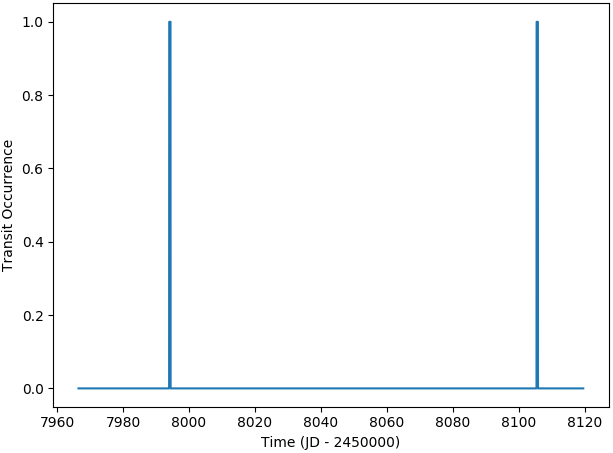
\includegraphics[width=0.8\textwidth]{transit.png}
\vspace{-1em}
\caption{The (primary) transit occurrence for HD 80606 during August-December 2017.}
\end{figure}


\section{Extreme Astrometry}
The VizieR and Simbad databases were used to get the right ascension (RA) and declination (DEC) of HD 80606, as well as its proper motion [5,6]. The uncertainties in GAIA for position, parallax, and proper motion were obtained directly from the ESA's DR1 website [7]. The code for this section can be found in \texttt{astrometry.py}. \texttt{astrometry\_planet()} accounts for the planet's influence on the star. It uses \texttt{projected\_separation\_com()} to find the star's offset with respect to the center of mass (caused by the planet's gravitational pull). It then converts this distance to angular separation, which is what is returned. \texttt{astrometry\_parallax()} accounts for the planet's and parallax's influence on the star. As earlier, the planet's influence is obtained using \texttt{astrometry\_planet()}. In order to obtain the influence of parallax, the effect of annual parallax on offset is calculated [8]. The RA and DEC are converted to ecliptic coordinates [9], and the Sun's ecliptic longitude is calculated [10]. This influence is then added to that from the planet to return the effect of the combined influence. \texttt{astrometry\_proper()} accounts for the planet's, parallax's, and proper motion's influence on the star. As earlier, the planet's and parallax's influences are obtained using \texttt{astrometry\_parallax()}. In order to obtain the influence of proper motion, we simply multiply the proper motion given from Simbad by the number of days passed. Because the RA and DEC used were for J2000, this is used as an offset to calculate the change that already occurred before the first time used in the program. This influence is then added to that from the planet and parallax to return the effect of the combined influence.

\begin{figure}[H]
\centering
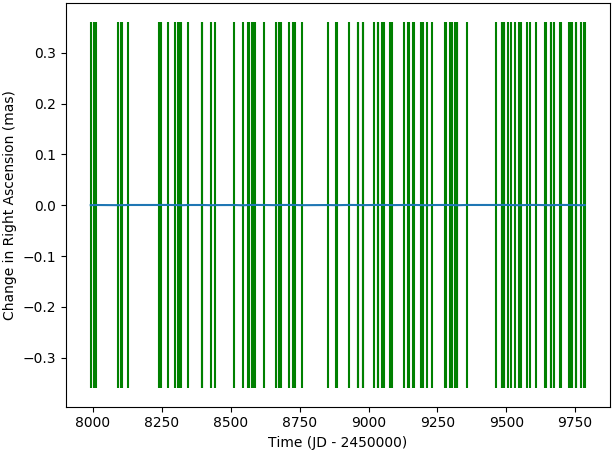
\includegraphics[width=0.75\textwidth]{planet_time_ra.png}
\vspace{-1em}
\caption{The time vs. RA graph for HD 80606's astrometry accounting for the planet's influence in 100 random epochs over a five-year period starting on August 1, 2017. Uncertainty from GAIA is shown in green.}
\end{figure}
\vspace{-1em}
\begin{figure}[H]
\centering
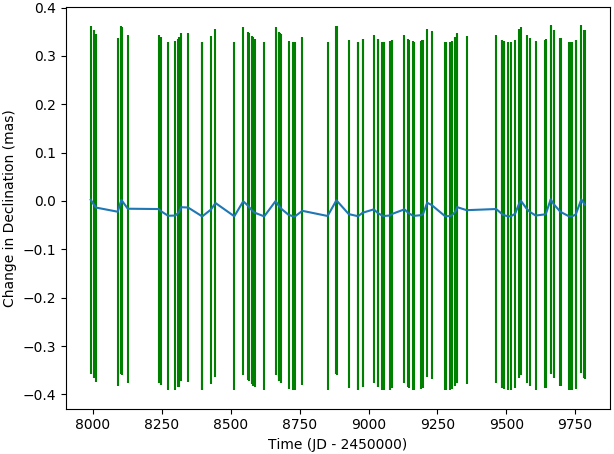
\includegraphics[width=0.75\textwidth]{planet_time_dec.png}
\vspace{-1em}
\caption{The time vs. DEC graph for HD 80606's astrometry accounting for the planet's influence in 100 random epochs over a five-year period starting on August 1, 2017. Uncertainty from GAIA is shown in green.}
\end{figure}
\vspace{-1em}
\begin{figure}[H]
\centering
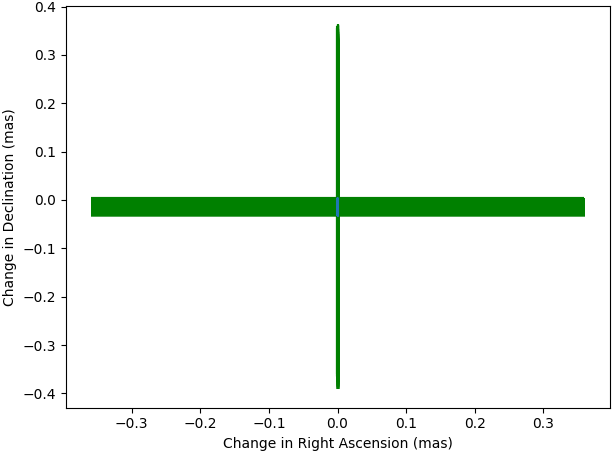
\includegraphics[width=0.75\textwidth]{planet_ra_dec.png}
\vspace{-1em}
\caption{The RA vs. DEC graph for HD 80606's astrometry accounting for the planet's influence in 100 random epochs over a five-year period starting on August 1, 2017. Uncertainty from GAIA is shown in green.}
\end{figure}
\vspace{-1em}
\begin{figure}[H]
\centering
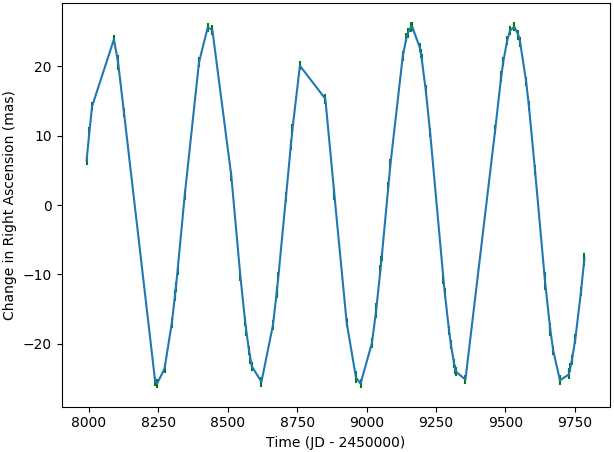
\includegraphics[width=0.75\textwidth]{parallax_time_ra.png}
\vspace{-1em}
\caption{The time vs. RA graph for HD 80606's astrometry accounting for the planet's and parallax's influences in 100 random epochs over a five-year period starting on August 1, 2017. Uncertainty from GAIA is shown in green.}
\end{figure}
\vspace{-1em}
\begin{figure}[H]
\centering
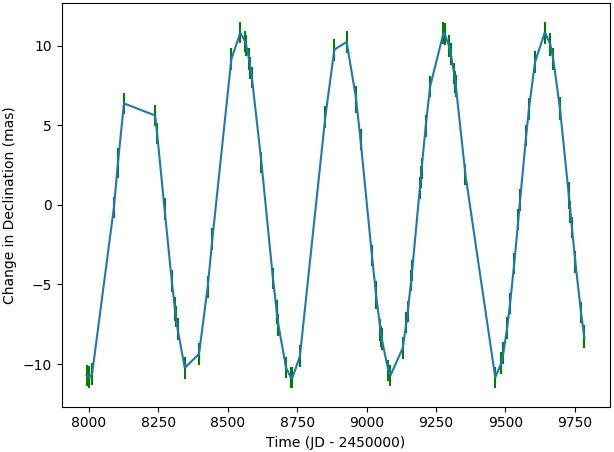
\includegraphics[width=0.75\textwidth]{parallax_time_dec.png}
\vspace{-1em}
\caption{The time vs. DEC graph for HD 80606's astrometry accounting for the planet's and parallax's influences in 100 random epochs over a five-year period starting on August 1, 2017. Uncertainty from GAIA is shown in green.}
\end{figure}
\vspace{-1em}
\begin{figure}[H]
\centering
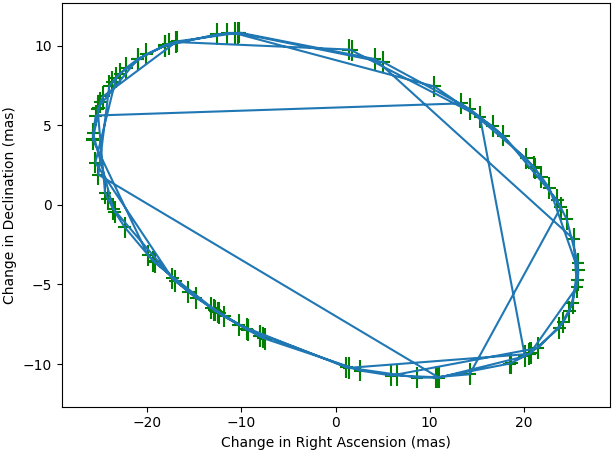
\includegraphics[width=0.75\textwidth]{parallax_ra_dec.png}
\vspace{-1em}
\caption{The RA vs. DEC graph for HD 80606's astrometry accounting for the planet's and parallax's influences in 100 random epochs over a five-year period starting on August 1, 2017. Uncertainty from GAIA is shown in green.}
\end{figure}
\vspace{-1em}
\begin{figure}[H]
\centering
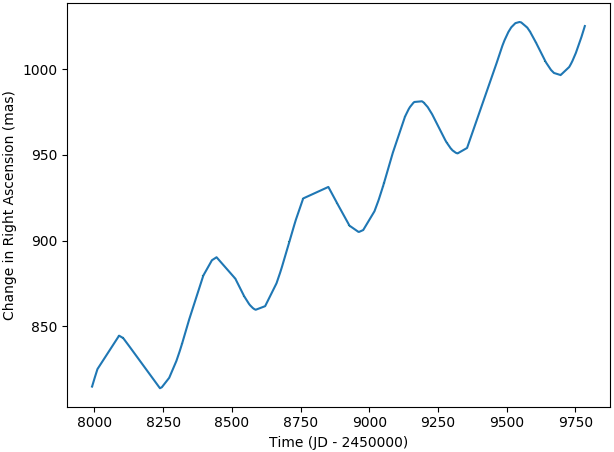
\includegraphics[width=0.75\textwidth]{proper_time_ra.png}
\vspace{-1em}
\caption{The time vs. RA graph for HD 80606's astrometry accounting for the planet's, parallax's, and proper motion's influences in 100 random epochs over a five-year period starting on August 1, 2017. Uncertainty from GAIA is shown in green.}
\end{figure}
\vspace{-1em}
\begin{figure}[H]
\centering
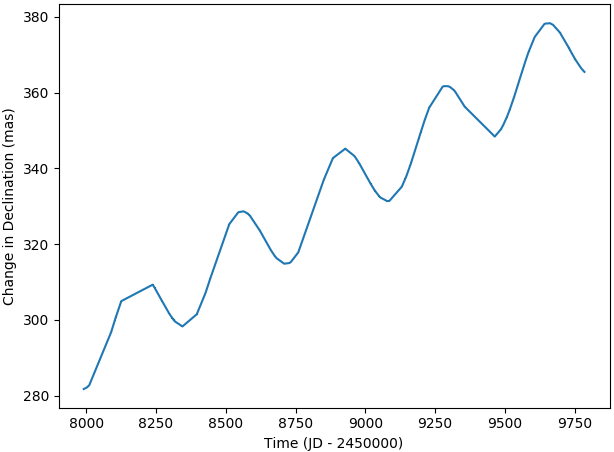
\includegraphics[width=0.75\textwidth]{proper_time_dec.png}
\vspace{-1em}
\caption{The time vs. DEC graph for HD 80606's astrometry accounting for the planet's, parallax's, and proper motion's influences in 100 random epochs over a five-year period starting on August 1, 2017. Uncertainty from GAIA is shown in green.}
\end{figure}
\vspace{-1em}
\begin{figure}[H]
\centering
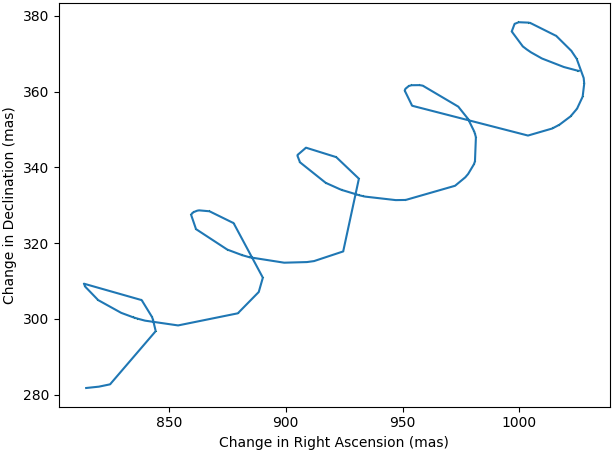
\includegraphics[width=0.75\textwidth]{proper_ra_dec.png}
\vspace{-1em}
\caption{The RA vs. DEC graph for HD 80606's astrometry accounting for the planet's, parallax's, and proper motion's influences in 100 random epochs over a five-year period starting on August 1, 2017. Uncertainty from GAIA is shown in green.}
\end{figure}


\section*{References}
\begin{mylist}
\item https://en.wikipedia.org/wiki/True\_anomaly
\item https://exoplanetarchive.ipac.caltech.edu/cgi-bin/DisplayOverview/nph-\\DisplayOverview?objname=HD+80606+b
\item http://snoopy.as.utexas.edu:8080/OS/sunrise-sunset-moon-calendar
\item http://www.briancasey.org/artifacts/astro/airmass.cgi
\item http://vizier.u-strasbg.fr/viz-bin/VizieR-5?-ref=VIZ59c6c0db54dc\&-out.add=.\&-source=\\III/135A/catalog\&recno=80606
\item http://simbad.u-strasbg.fr/simbad/sim-id?Ident=HD\%2080606
\item https://www.cosmos.esa.int/web/gaia/dr1
\item http://star-www.st-and.ac.uk/\textasciitilde{}fv/webnotes/chapt14.htm
\item https://github.com/Caltech-IPAC/Montage/blob/master/lib/src/coord/convertEclEqu.c
\item http://aa.usno.navy.mil/faq/docs/SunApprox.php
\end{mylist}


\end{document}